% !TeX spellcheck = en_GB
% !TeX encoding = UTF-8
% !TeX root = ../thesis.tex
\chapter{N-Gram Bug Detection in \scratch{}}\label{chap:methods}
%TODO Unfinished chapter!

\begin{figure}[hbtp]
\centering
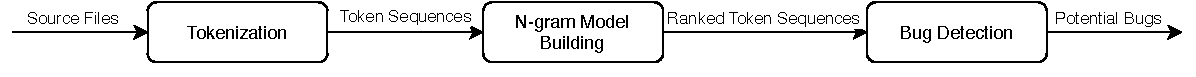
\includegraphics[scale=0.75]{images/Overview.pdf}
\caption{Overview of the n-gram model building process}
\label{fig:overview}
\end{figure}

Figure \ref{fig:overview} visualizes the \ngram{} building process which is explained in this chapter in more detail. In Section~\ref{sec:tokenization} the tokenization process is described with the way the \scratch{} project is parsed and converted into tokens. The next step is to use the created tokens to build the \ngram{} like it is shown in Section~\ref{sec:model}. Finally, bugs can be detected with the help of the calculated model according to Section~\ref{sec:detection}.

\section{Tokenization of \scratch{} Code}\label{sec:tokenization}
In order to build a model, we need to tokenize the \scratch{} project into suitable pieces:

\begin{definition}[Token]\label{def:token}
    %
    ``A token is a single fragment of \scratch{} code that is used to partition code into smaller pieces in order to obtain information about its syntax on a specific granularity level.''
    %
\end{definition}

%TODO Edit this part for better understanding
It is hard to find the right granularity, but it is important that the whole project can be represented by tokens, so that unusual blocks can be identified. To visualize a \scratch{} project, the tokenization process is based on the Abstract Syntax Tree (\AST{}) structure of \litterbox{}. 
For a simple start, the best way to break the project apart is to identify all drag-and-drop blocks that everyone is familiar with from \scratch{}. After isolating all bigger blocks, the question is how in depth the analysis should be. In this bachelor's thesis the focus is on all literals and variables that can be manipulated by the \scratch{} programmer. This approach lead to the exclusion of all kinds of \AST{}Nodes that only exist for initialization purposes, metadata or even blocks that can only be chosen in a drop-down menu inside a block.  

\section{N-gram Model Building in \scratch{}}\label{sec:model}
In the following sections the focus is the building process of the \ngram{}, specifically in \scratch{}. Subsection~\ref{subsec:n-grams} goes in detail on how to calculate the probabilities of the found token sequences and add them to the growing model. The method of Smoothing is then explained in Subsection~\ref{subsec:smoothing} as well as its importance in bug detection.

\subsection{Calculating and Adding N-grams}\label{subsec:n-grams}
First of all, the language model has to extract all possible token sequences in a \scratch{} project and calculate their probabilities like it is described in Subsection~\ref{subsec:n-grams}. This way a good probability distribution is created that will be the basis for later bug detection. 

For example, given the sequence [GreenFlag, Show, Hide] that is shown in Figure~\ref{fig:sequence}, all its consecutive subsequences are added to the model. In this case the subsequence [GreenFlag, Hide] in Figure~\ref{fig:subsequence} would be the only sequence that is ignored because [Hide] does not immediately follow [GreenFlag]. 

\begin{figure}%
    \centering
    \subfloat[A \scratch{} block sequence]{{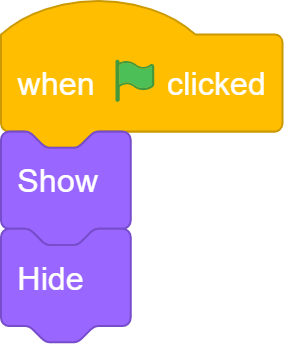
\includegraphics[width=5cm]{sequence.png} }\label{fig:sequence}}%
    \qquad
    \subfloat[Ignored subsequence]{{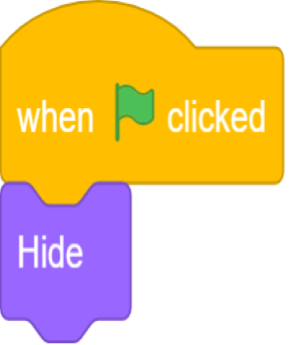
\includegraphics[width=5cm]{subsequence.png} }\label{fig:subsequence}}%
    \caption[\scratch{} block sequences]{\label{fig:sequences}\scratch{} block sequences}%
\end{figure}

If Figure~\ref{fig:sequence} would be the sequence we want to calculate the probability of, the estimation based on the \hyperref[def:markov_chain]{Markov chain} is executed by solving the Equation~\ref{eq:scratch-prob}. We are setting the \hyperref[def:gram size]{gram size} to 3 in this example. All internal probabilities are added by consulting the existing model and searching for the already calculated estimations. Therefore, the token sequence [GreenFlag, Show, Hide] can be calculated based on internal probabilites of its existing subsequences.

\begin{equation} \label{eq:scratch-prob}
\begin{aligned}
P([GreenFlag, Show, Hide]) ={} & P([GreenFlag])\cdot P([Show]|[GreenFlag]) \\
							  & \cdot P([Hide]|[GreenFlag, Show])
\end{aligned}
\end{equation}


\subsection{Smoothing of Probability Distribution}\label{subsec:smoothing}
If the analysed project is not part of the training dataset, it is important to smooth the probability distribution in order to avoid probabilities of zero. In this implementation, Add-One-Smoothing was utilized which prevents non existent sequences to be shown by adding an additional count to each n-gram.
All the counts that used to be zero will now have a count of 1, the counts of 1 will be 2, and so on. This algorithm is also called Laplace smoothing. This way there are no sequences with a probability of zero stored in the model that could affect the calculation of the sequence probabilities.

In the case of the unigram [GreenFlag], its maximum likelihood to appear in a \scratch{} project is estimated by counting the occurrences \textit{c} during the model training process and divide it through the total number of tokens \textit{N}. Therefore, the Equation~\ref{eq:likelihood} looks like this:

\begin{equation} \label{eq:likelihood}
P([GreenFlag]) ={} \frac{c}{N}
\end{equation}

Add-One Smoothing then, like the name suggests, only adds one to each count. Since there are a total of \textit{V} tokens in the model vocabulary and we added one more sighting to each one of them, we also have to adjust the denominator of the fraction accordingly. One more observation of each token means we have to increase the denominator by \textit{V}. If we apply the Math rules, the equation results in the following calculation in Equation~\ref{eq:laplace}:

\begin{equation} \label{eq:laplace}
P_{Laplace}([GreenFlag]) ={} \frac{c + 1}{N + V}
\end{equation}


\section{Bug Detection in \scratch{}}\label{sec:detection}
The specific algorithm to find bugs in \scratch{} is implemented the following way. At first, the probabilities of all sequences of the analysed project have to be calculated with help of the model like it is described in Subsection~\ref{subsec:n-grams}. After that, based on their probability the sequences are ranked and only the ones with the lowest probability get reported as potential bugs. In the next Subsection~\ref{subsec:configurations} all important parameters are set to ensure the optimal model analysis results. In Subsection~\ref{subsec:false_bugs} we found a method to minimize the amount of false positives in the reported bug set.

\subsection{Configurations}\label{subsec:configurations}
%TODO Further explanation for parameters
For the \scratch{} model implementation we added five parameters that have to be set accordingly in order to achieve the best evaluation results that are discussed later in Chapter~\ref{chap:evaluation}.

\paragraph{Gram Size.}
For probability calculations a \hyperref[def:markov_chain]{Markov chain} is used to get the conditional probability of a sequence using its n-1 token predecessors as context information. In this work, I built n-gram models with a gram size between 2 to 6 in order to find the optimal n for bug detection in \scratch{} projects (Section \ref{sec:gram_size}). 
\paragraph{Sequence Length.}
In the same way I used a large dataset to obtain information about the best \hyperref[def:gram_size]{gram size n}, I also analysed which length of a token sequence could be the optimal size for a good model. Finding the right length of a token sequence is evaluated in a more detailed way in Section \ref{sec:sequence_length}.
\paragraph{Reporting Size.}
In this implementation the reporting size is fixed at 25 reports per analysis. 
\paragraph{Minimum Token Occurrence.}
In this bachelor's thesis \ngram{} which is only for \scratch{} analysis purposes the minimum token occurrence is chosen as one. Because of the size difference between usual Java projects compared to normal \scratch{} projects, it would not make sense to filter out any tokens. \scratch{} programmers do not have as much freedom in their implementation because of the restriction through a block-based language and usually choose a different purpose for their programs than text-based programming languages would, which leads to much smaller projects with fewer usages of specific tokens. So, the minimum token occurrence parameter would only make it harder to find low probability sequences in projects which is why I decided not to raise this threshold for my analysis.
\paragraph{Probability Threshold.}
If a sequence in the report has a probability that is higher than the given threshold, it probably is a normal token sequence that just happens to have a lower probability than the rest of the project's blocks. In this implementation, the threshold is fixed at 0.05.

\subsection{Pruning False Bugs}\label{subsec:false_bugs}
Token sequences with low probability are at the bottom of a n-gram reporting list for potential bugs. But there is always the chance that the found sequence is not actually wrong but just a very unusual or special use case in which its probability would also rank rather low. To find and filter out this kind of false bugs and reduce the candidate bug set, token sequences can only be reported when they are at the bottom of at least two ranked lists of \ngram{s} with the same \textit{gram size} but different \textit{sequence lengths}. This way, sequences are sorted out that just appear on one of these lists and the chance to report false positives gets drastically reduced. 